\documentclass[12pt,a4paper]{report}
\usepackage[utf8]{inputenc}
\usepackage{amsmath}
\usepackage{amsfonts}
\usepackage{amssymb}
\usepackage{graphicx}
\usepackage{listings}
\usepackage{fancyhdr}
\usepackage{parskip}
\usepackage{rotating}
\usepackage{caption}
\usepackage{subcaption}

\pagestyle{fancy}
\chead{2.1.10 - sw608f14 - Daniel S. F., Lars A, Mathias W. P. \& Søren S. A.}

\lstset{mathescape = true}
\usepackage{amsthm}
\begin{document}
\section*{Selfstudy 4}
\section*{17-2}
Was answered in last self-study.

\section*{33-1}
\subsection*{a.}
We can use Jarvis's march until Q is empty.  Its cost is $O(n*h)$, so if we run it several times for j layers such that all points have been wrapped in a layer the cost will be $O(n*h_1 + n*h_2 .... n*h_j$. And we have $\sum\limits_{i=0}^j{h_i} = n$. So the worst case running time will be $O(n^2)$

\subsection*{b.}
Proof by contradiction.
First we see how we could use a convex layers algorithm to sort real numbers.
We could make the n real numbers into points where their x coordinate is their real number value and the y coordinate is 0.
This would result in the real numbers being chained and could be outputted in the correct order in $n$ time after being chained.
so if we had an algorithm for the convex layers problem that could run faster than $n*lg(n)$ we would  be able to sort faster than $n*lg(n)$ which is impossible.

\section*{33-2}
\subsection*{a.}
We observe that $y_i$ is the maximal $y$ value for the $i$'th layer, as if it was not the maximal $y$ value, it would be dominated by the other points in the layer, as they already have a higher x value.
We then take a look at $y_i$ and $y_{i+1}$ we already know that $y_i \geq y_{i+1}$ but it cannot be equal, because then the point the $y_{i+1}$ value is connected to would be in the $i$'th layer. So we have that $y_{i} > y_{i+1}$.
And thus $y_1 > y_2 > ... > y_k$

\subsection*{b.}
To understand the cases better, we first draw a sketch.

\begin{figure}[h]
        \centering
        \begin{subfigure}[b]{0.4\textwidth}
                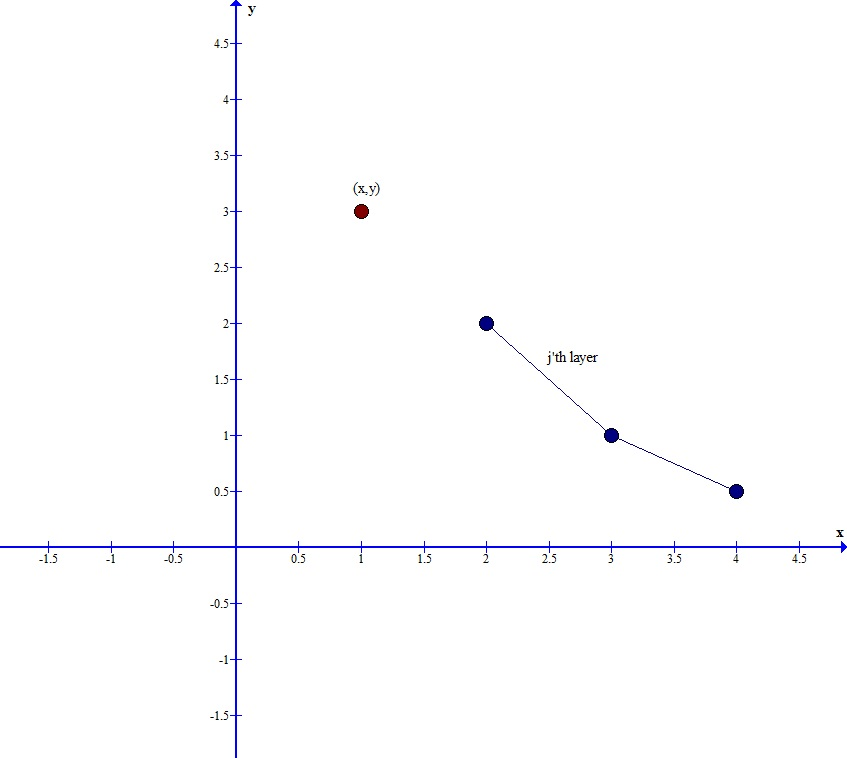
\includegraphics[width=\textwidth]{332graph1}
                \caption{Case 1}
                \label{fig:graph1}
        \end{subfigure}
        ~
        \begin{subfigure}[b]{0.4\textwidth}
                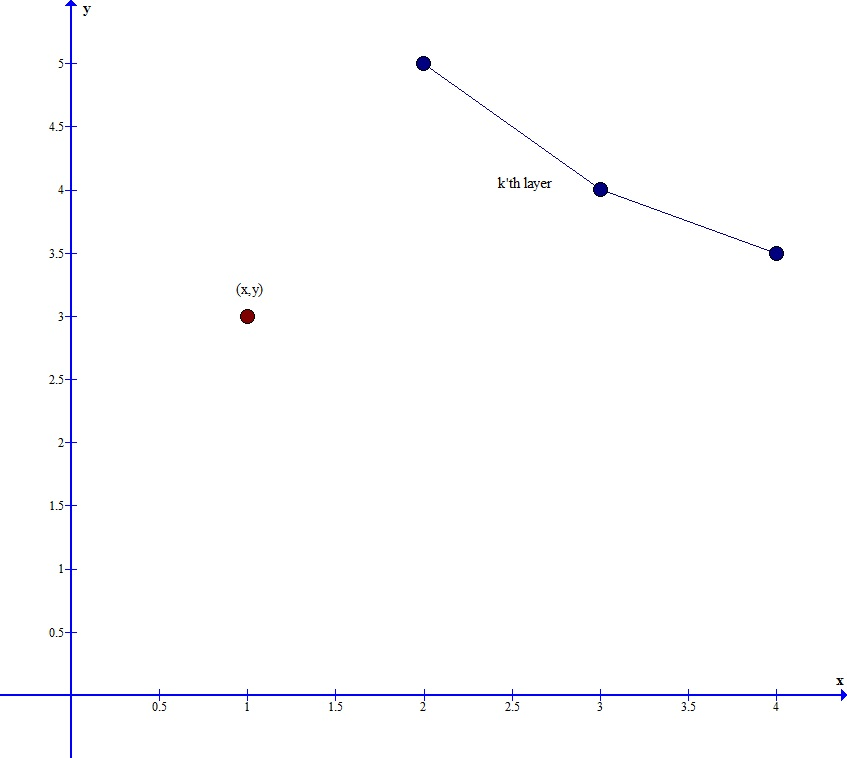
\includegraphics[width=\textwidth]{332graph2}
                \caption{Case 2}
                \label{fig:graph2}
        \end{subfigure}

\end{figure}

As can be seen, Figure \ref{fig:graph1} shows the case where the left most point can stay in the $j'th$ layer.
Whereas Figure \ref{fig:graph2} shows where a new layer $k+1$ with the point have to be added.

To show it, we know that $(x,y)$ is the leftmost point.

For $j \leq k$:
As we know that $(x,y)$ is the leftmost point we know that it does not dominate any other points. But we know that $y_j < y$ and so we know that $(x,y)$ is not dominated by any points in the $j'th$ layer and thus $(x,y)$ should be added to the $j'th$ layer.

For $j=k+1$:
We already know that $(x,y)$ is the leftmost point. $y_k$ is the leftmost point of the $k'th$ layer, which is the last layer, and as we know that $y<y_k$ it cannot be in the $k'th$ layer as it would then be dominated by other points in that layer, we need a new layer $k+1$ containing the point $(x,y)$.

  
\subsection*{c.}

\begin{lstlisting}
Algo(Q:set of n points)
   Sort(Q) //on x value decending
   
   for i = 0 to n
      if A is empty
         A[0].add(Q[i])
      else
         Binary search A to find j.
         if Q[i].y < A.last.y
            A.addlayer
            A.last.add(Q[i])                  
         else
            A[j].add(Q[i])
\end{lstlisting}
And so binary search costs $O(lg(n))$ and the loop runs $n$ times, so we have a running time of $O(n*lg(n))$

\subsection*{d.}
Difficulties do arise with same x or same y coordinate. To solve the issue with same x coordinate, we ensure that we sort $Q$ by x value descending and then \textit{by y value descending}.
For the same y coordinate we change the condition $y < y_k$ to be $y \leq y_k$.


\end{document}